\documentclass[a4paper, twoside, english]{article}

\usepackage{amsmath}
\usepackage{amsfonts}
\usepackage{ihci}
\usepackage{graphicx}
\usepackage{subfig}

\graphicspath{{./figures/}}

\title{Exercise 4}
\author{
	Abdelaziz, Ibrahim
	\and
	Somkiadcharoen, Robroo
	\and
	Berg, Oliver
}
\date{\today}

\begin{document}
\maketitle


\section{Theory}

\subsection{T1}
After images Rectification all points correspondences lie on the same scan horizontal line parallel to the baseline, which simplifies the search to a 1D horizontal search.

\subsection{T2}
In rectified image pair traingulation is reduced to simple geometric problem where correspondence points' depth can be calculated using this simple equation \begin{equation} Z = f.t_{x} \div disparity \end{equation}
\subsection{T3}
Image rectification for multi-view dense reconstruction may produce information loss, because all images are projected to a plane where all cameras are parallel, which is not a valid approximation in case of the given example where several images were taken around a statue.  

\section{Implementation}
\subsection{I1}
The disparity map is not a good representation of the original scene, because the Pixel-based matching used is not accurate, and the best match found for each point is not necessarily its real correspondence. 
\subsection{I2}
NCC-based matching is more accurate than Pixel-base matchig, because it uses a window to search for correspondences, and hence the resulting disparity map is better that the Pixel-based one.

\subsection{I3}

Figure 1 contains images of two reconstructed point clouds: 

\begin{figure}[ht]
 \centerline
 {
  \subfloat[]{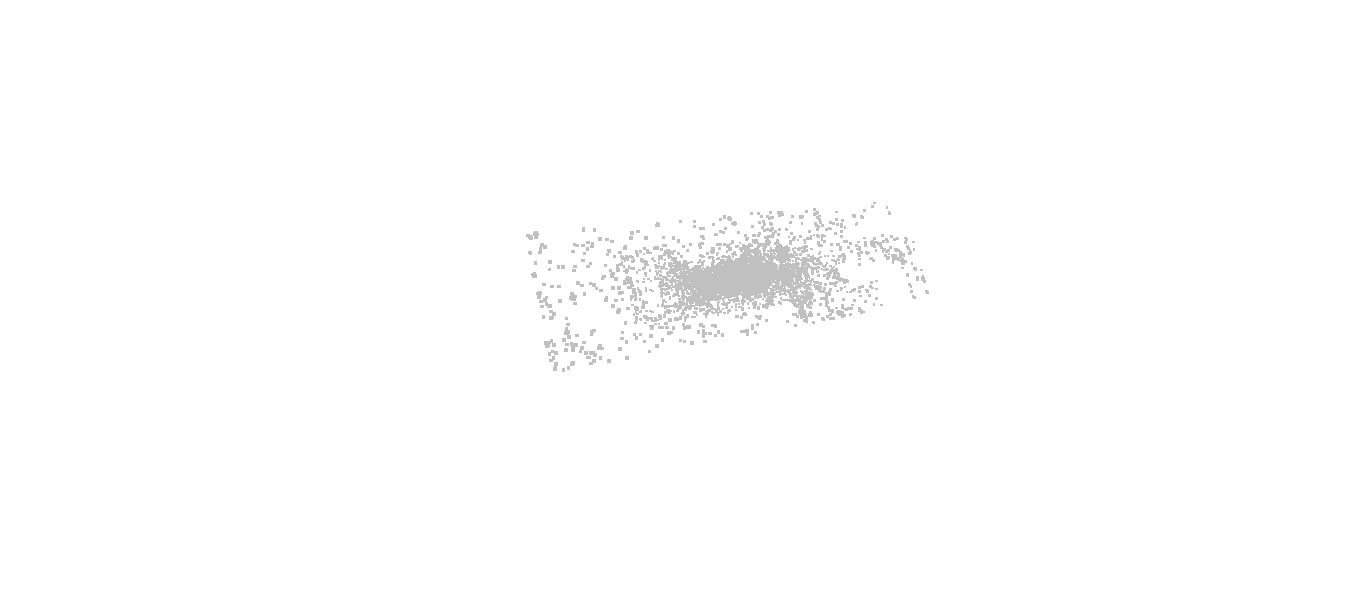
\includegraphics[width=0.35\textwidth]{pixel_based.png}}
  \qquad
  \subfloat[]{
\includegraphics[width=0.35\textwidth]{ssd_7_based.png}}
 }
 \caption[Color inversion]{(a) pixel-based Matching. (b) SSD-based Matching window size 7.}
 \label{fig:inversion}
\end{figure}

\subsection{I4}
With tried window sizes of 3,5,7. Window of size 7 yields the best disparity map in this case, because matching errors are decreased with larger window size.

\subsection{Q1}
Increasing the window size increases reconstruction quality, because matching errors is decreased.
\subsection{Q2}
Increasing the window size increases the processing time greatly. Since points correspondence search is independent on other points we can parallelize the Implementation and use GPUs to decrease the processing time. 

\end{document}
